\chapter{Sports and Categories}

\section{Overview of Paralympic Sports}

\subsection{A Tapestry of Disciplines: Showcasing Diverse Abilities}

The Paralympic Games, a parallel event to the Olympic Games, celebrate the remarkable athleticism and achievements of individuals with disabilities across a wide spectrum of sports.  These Games showcase a diverse tapestry of disciplines, ranging from the explosive power of wheelchair rugby and the precision of archery to the strategic brilliance of wheelchair fencing and the graceful elegance of para-equestrian dressage.  Paris 2024 is set to feature 22 sports and over 500 events, offering a captivating spectacle of skill, determination, and sportsmanship that will inspire and excite audiences worldwide.

\subsection{Leveling the Playing Field: The Classification System}

Central to the Paralympic Games is a meticulous classification system designed to ensure fair and equitable competition.  This system groups athletes based on the impact of their impairment on their athletic performance, fostering an environment where individuals with different impairments can compete against others with similar functional abilities. By leveling the playing field, the classification system highlights the unique skills, strategies, and adaptations that each athlete brings to their chosen sport. The classification process is rigorous and ongoing, with experts evaluating athletes' functional abilities to ensure they are placed in the most appropriate categories, thus maximizing their potential and showcasing their true talents.

\section{Paralympic Sports}

\subsection{Archery}

\begin{enumerate}

\item Essence of Archery
    \begin{itemize}
    \item Paralympic archery is a test of precision, control, and mental focus, where athletes with various impairments compete to hit a target with a bow and arrow. 
    \item It requires incredible concentration and steady hands, as even the slightest movement can affect the trajectory of the arrow. 
    \item To ensure fair competition and enable athletes with different abilities to participate, Paralympic archery incorporates a range of adaptive equipment, including wheelchairs, stools, and mouth tabs for those with limited arm or hand function.
    \end{itemize}

\begin{figure}[htbp] % htbp are float placement options
\centering
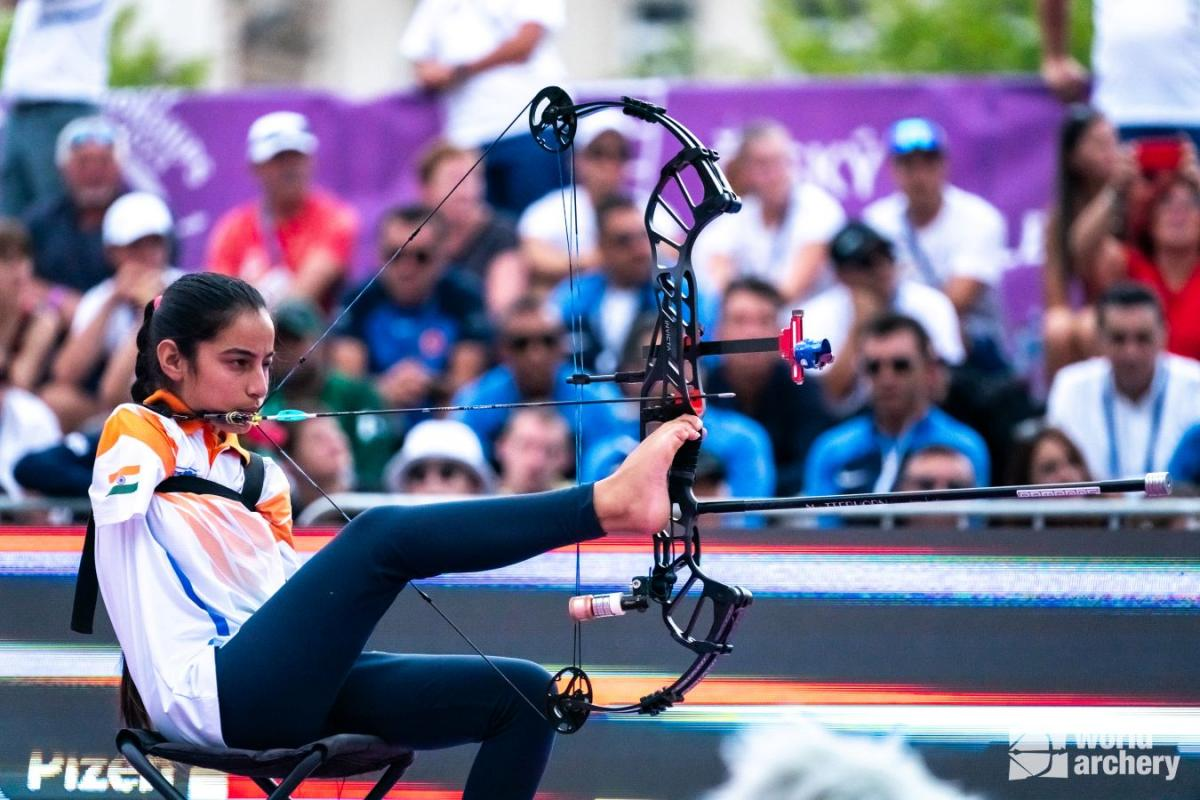
\includegraphics[width=0.8\textwidth]{Images/para_archery.jpg}
\caption{Para Archery}
\label{fig:my_image}
\end{figure}

\item Rules, Equipment, and Competition
    \begin{itemize}
    \item Paralympic archery follows similar rules to Olympic archery, with athletes aiming to score the highest points by hitting the center of a target at various distances. 
    \item Recurve bows and compound bows are the two main types used, and athletes can use assistive devices based on their classification. 
    \item Competition formats include individual, team, and mixed events, adding to the excitement and showcasing the diverse talents of Paralympic archers.
    \end{itemize}

\item Categories and Classifications
    \begin{itemize}
    \item Paralympic archery utilizes a classification system based on the athlete's physical impairment. 
    \item There are three main categories: 
        \begin{itemize}
        \item W1 for athletes with significant limitations in their upper and lower limbs
        \item W2 for those with impairments primarily affecting their lower limbs
        \item Open for athletes with less severe impairments
        \end{itemize}
    \item The classification system ensures that athletes compete against others with comparable functional abilities, fostering fairness and enabling everyone to reach their full potential in the sport.
    \end{itemize}

\end{enumerate}
\subsection{Athletics}

\begin{enumerate}

\item Essence of Athletics
    \begin{itemize}
    \item Paralympic athletics encompasses a wide range of track, field, and road events, pushing athletes with various impairments to the limits of their physical capabilities. 
    \item It's a showcase of speed, power, endurance, and technical skill, with athletes competing in events like sprints, long jump, discus throw, and marathons. 
    \item Paralympic athletics demonstrates the extraordinary feats that can be achieved through dedication, training, and the unwavering pursuit of personal bests.
    \end{itemize}

\item Rules, Equipment, and Competition
    \begin{itemize}
    \item Paralympic athletics adheres to the fundamental rules of athletics, with adaptations made to accommodate different impairments. 
    \item Athletes can utilize adaptive equipment such as racing wheelchairs, running blades, and throwing frames to maximize their performance. 
    \item Competitions typically involve heats, semifinals, and finals, creating a thrilling atmosphere as athletes strive for podium finishes and record-breaking performances.
    \end{itemize}

\item Categories and Classifications
    \begin{itemize}
    \item Paralympic athletics employs a complex classification system that takes into account various impairments, including visual, physical, and intellectual disabilities. 
    \item Athletes are assessed based on their functional abilities, ensuring fair competition among those with similar levels of impairment. 
    \item This system uses a combination of letters and numbers to categorize athletes, such as T/F classes for track and field events, allowing spectators to understand the specific classifications and appreciate the unique challenges and achievements of each athlete.
    \end{itemize}
\end{enumerate}
\subsection{Badminton}

\begin{enumerate}

\item Essence of Badminton
    \begin{itemize}
    \item Paralympic badminton is a fast-paced and dynamic sport that showcases the agility, reflexes, and tactical acumen of athletes with various impairments.
    \item It involves hitting a shuttlecock over a net using a racket, demanding quick movements, precise shots, and strategic gameplay. 
    \item The sport offers both singles and doubles competitions, providing opportunities for athletes to demonstrate their individual skills and teamwork.
    \end{itemize}

\item Rules, Equipment, and Competition
    \begin{itemize}
    \item Paralympic badminton follows the core rules of badminton, with modifications made to accommodate different impairments. 
    \item Athletes can compete in standing or wheelchair categories, and the court dimensions and net height might be adjusted for certain classifications. 
    \item The competition format typically includes group stages followed by knockout rounds, culminating in exciting finals where athletes battle for medals and glory.
    \end{itemize}

\item Categories and Classifications
    \begin{itemize}
    \item Paralympic badminton employs a classification system based on the athlete's physical impairment, ensuring fair competition among those with similar functional abilities. 
    \item The system uses a combination of letters and numbers to categorize athletes, such as WH for wheelchair users and SL for standing lower limb impairments. 
    \item The classifications consider factors like muscle power, range of movement, and balance, allowing athletes to compete against others with comparable levels of impairment and showcase their badminton skills.
    \end{itemize}

\end{enumerate}
\subsection{Boccia}

\begin{enumerate}

\item Essence of Boccia
    \begin{itemize}
    \item Boccia, a precision ball sport, is a captivating display of strategy, accuracy, and finesse.
    \item Athletes with severe physical impairments, often using wheelchairs or assistive devices, compete by propelling or rolling balls towards a target ball, aiming to get their balls closest to the target.
    \item It's a game of tactics and control, requiring players to carefully assess the playing field and execute their throws with precision. 
    \end{itemize}

\item Rules, Equipment, and Competition
    \begin{itemize}
    \item Boccia is played on a flat, rectangular court, with athletes taking turns throwing or rolling their balls towards the target. 
    \item The game can be played individually, in pairs, or in teams, and points are awarded based on the proximity of each ball to the target. 
    \item The sport uses specially designed balls and assistive devices, such as ramps and head pointers, to enable athletes with various impairments to participate fully.
    \end{itemize}

\begin{figure}[htbp] % htbp are float placement options
\centering
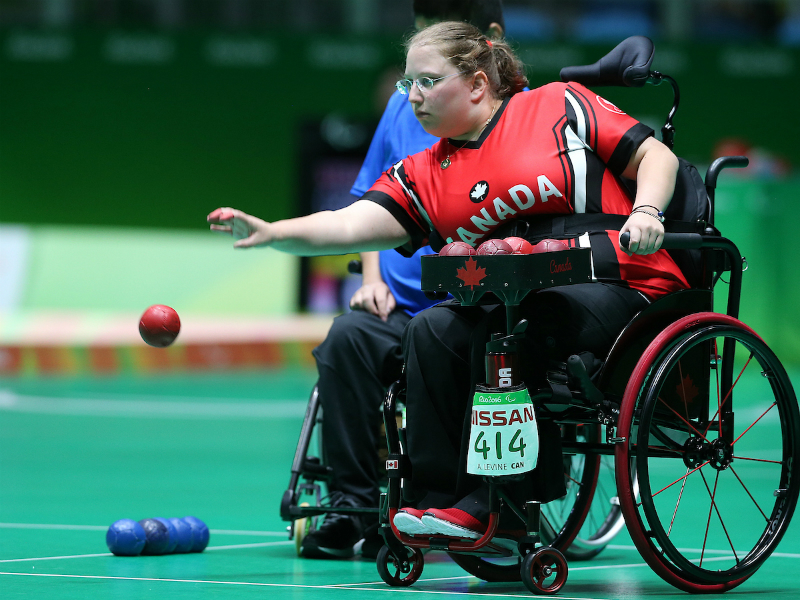
\includegraphics[width=0.8\textwidth]{Images/para_bocce.jpg}
\caption{Para Bocce}
\label{fig:my_image}
\end{figure}

\item Categories and Classifications
    \begin{itemize}
    \item Boccia has a classification system that groups athletes based on the severity of their physical impairments. 
    \item There are four main classifications:
        \begin{itemize}
        \item BC1 for athletes who can throw or kick the ball
        \item BC2 for those who can throw the ball but require assistance with positioning
        \item BC3 for those who cannot throw or kick the ball and use a ramp to propel it
        \item BC4 for athletes with other impairments affecting their coordination and movement
        \end{itemize} 
    \item This system ensures fair competition and allows athletes with diverse abilities to demonstrate their skills and strategies in the sport.
    \end{itemize}

\end{enumerate}
\subsection{Canoe (Para Canoe)}

\begin{enumerate}

\item Essence of Canoe
    \begin{itemize}
    \item Paralympic canoe, also known as para-canoe, is a thrilling water sport that showcases the strength, endurance, and paddling technique of athletes with physical impairments. 
    \item It involves paddling a canoe or kayak over a set distance, demanding a combination of upper body power, core stability, and precise boat control. 
    \item The sport offers both sprint and long-distance events, providing opportunities for athletes to excel in different paddling disciplines.
    \end{itemize}

\item Rules, Equipment, and Competition
    \begin{itemize}
    \item Paralympic canoe follows similar rules to Olympic canoe, with modifications made to accommodate different impairments. 
    \item Athletes compete in various boat classes, including kayaks (K) and va'a (V), and the competition format typically involves heats and finals. 
    \item The sport utilizes adaptive equipment, such as specialized seats and paddles, to ensure athletes with various impairments can participate safely and effectively.
    \end{itemize}

\item Categories and Classifications
    \begin{itemize}
    \item Paralympic canoe employs a classification system based on the athlete's physical impairment, ensuring fair competition among those with similar functional abilities. 
    \item The system uses a combination of letters and numbers to categorize athletes, such as KL for kayak lower limb impairments and VL for va'a lower limb impairments. 
    \item The classifications consider factors like muscle power, trunk function, and balance, allowing athletes to compete against others with comparable levels of impairment and demonstrate their paddling prowess.
    \end{itemize}

\end{enumerate}
\subsection{Cycling}

\begin{enumerate}

\item Essence of Cycling
    \begin{itemize}
    \item Paralympic cycling is a thrilling display of speed, endurance, and technical skill, featuring athletes with various impairments competing on bicycles, tricycles, handcycles, or tandems.
    \item The sport encompasses a range of disciplines, including road races, time trials, track cycling, and mountain biking, offering opportunities for athletes to excel in different cycling styles and terrains. 
    \end{itemize}

\item Rules, Equipment, and Competition
    \begin{itemize}
    \item Paralympic cycling follows similar rules to Olympic cycling, with adaptations made to accommodate different impairments. 
    \item Athletes compete in different classes based on their impairment and the type of bike they use. Competitions can be individual or team events, and they involve various formats such as time trials, road races, and pursuit races. 
    \item Adaptive equipment plays a crucial role, with specialized bikes, handcycles, and tandems enabling athletes to participate and compete at their best.
    \end{itemize}

\item Categories and Classifications
    \begin{itemize}
    \item Paralympic cycling uses a comprehensive classification system based on the athlete's impairment and functional abilities. 
    \item The system considers factors such as muscle power, range of movement, coordination, and vision. 
    \item Athletes are categorized into different classes, such as C for cyclists with physical impairments and B for visually impaired cyclists who compete on tandems with a sighted pilot. 
    \item This classification ensures fair competition and allows athletes to compete against others with comparable levels of impairment.
    \end{itemize}

\end{enumerate}
\subsection{Equestrian (Para-Dressage)}

\begin{enumerate}

\item Essence of Equestrian
    \begin{itemize}
    \item Paralympic equestrian, also known as para-dressage, is a graceful and elegant sport that highlights the harmony between horse and rider. 
    \item Athletes with physical impairments showcase their skill, balance, and communication with their equine partners as they perform a series of intricate movements and patterns. 
    \item This sport demonstrates the unique bond between humans and animals and the transformative power of therapeutic riding.
    \end{itemize}

\item Rules, Equipment, and Competition
    \begin{itemize}
    \item Paralympic equestrian is governed by the rules of the International Equestrian Federation (FEI), with adaptations for athletes with impairments. 
    \item Competitions involve individual and team events, with riders performing dressage tests at different levels of difficulty. 
    \item Horses are carefully selected and trained, and adaptive equipment such as mounting blocks and specialized saddles may be used to assist riders with specific needs.
    \end{itemize}

\item Categories and Classifications
    \begin{itemize}
    \item Paralympic equestrian uses a classification system based on the rider's physical impairment and functional abilities. 
    \item There are five grades, ranging from Grade I for riders with the most severe impairments to Grade V for those with minimal impairments. 
    \item The classification process assesses factors like muscle strength, coordination, balance, and vision, ensuring that riders compete against others with similar functional abilities.
    \end{itemize}

\end{enumerate}
\subsection{Football 5-a-side}

\begin{enumerate}

\item Essence of Football 5-a-side
    \begin{itemize}
    \item Football 5-a-side, a sport specifically designed for athletes with visual impairments, is a thrilling and fast-paced game that relies on sound and touch. 
    \item Players, except for the goalkeeper, are blindfolded and use a ball with a bell inside to navigate and score goals. 
    \item The sport showcases exceptional spatial awareness, ball control, and teamwork, as players rely on communication and trust to succeed.
    \end{itemize}

\item Rules, Equipment, and Competition
    \begin{itemize}
    \item Football 5-a-side is played on a smaller field with sideboards to keep the ball in play. 
    \item Each team consists of four outfield players and a sighted goalkeeper. 
    \item The game is played in two 25-minute halves, and players must shout "Voy!" when approaching the ball to avoid collisions. 
    \item The sport utilizes a special ball with a bell and requires players to wear eyeshades to ensure a level playing field.
    \end{itemize}

\item Categories and Classifications
    \begin{itemize}
    \item All outfield players in football 5-a-side are classified as B1, meaning they have very low visual acuity or no light perception. 
    \item The goalkeeper, however, can be fully or partially sighted. 
    \item This classification ensures fair competition and highlights the remarkable skills and adaptations of athletes with visual impairments in navigating and playing the game.
    \end{itemize}

\end{enumerate}
\subsection{Goalball}

\begin{enumerate}

\item Essence of Goalball
    \begin{itemize}
    \item Goalball, a unique team sport designed for athletes with visual impairments, is a thrilling contest of agility, accuracy, and sound perception. 
    \item Players, all blindfolded, attempt to roll or throw a ball with bells embedded into the opposing team's goal, while their opponents try to block the ball using their bodies. 
    \item The sport demands exceptional hearing, spatial awareness, and teamwork, creating an intense and exciting atmosphere.
    \end{itemize}

\item Rules, Equipment, and Competition
    \begin{itemize}
    \item Goalball is played on a court with tactile markings, and each team consists of three players. 
    \item The game is played in two 12-minute halves, and players must roll or throw the ball along the ground to score. 
    \item The ball has bells inside to allow players to track its movement, and players must remain silent during the game to enhance their hearing. 
    \item The sport showcases the incredible adaptability and athleticism of athletes with visual impairments.
    \end{itemize}

\begin{figure}[htbp] % htbp are float placement options
\centering
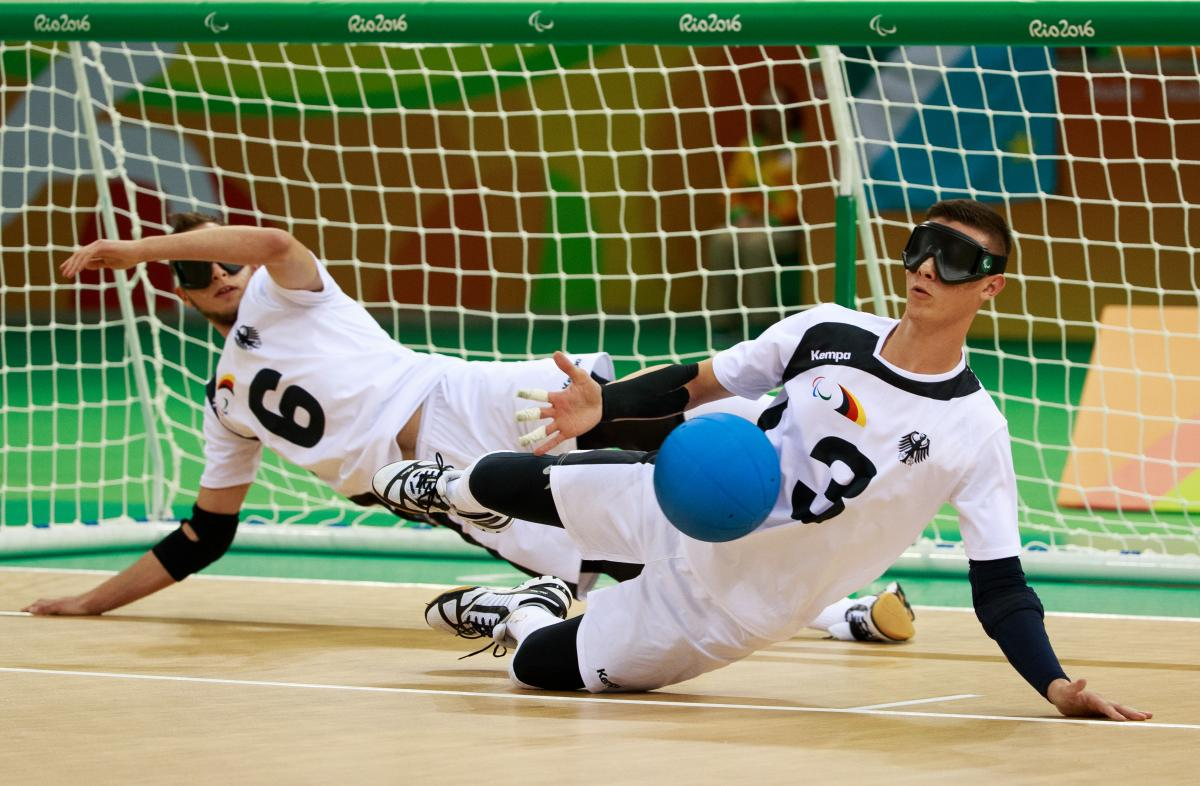
\includegraphics[width=0.8\textwidth]{Images/goalball.JPG}
\caption{Goalball}
\label{fig:my_image}
\end{figure}

\item Categories and Classifications
    \begin{itemize}
    \item All players in goalball are classified as B1, B2, or B3, based on the severity of their visual impairment. B1 players have the least visual acuity, while B3 players have the most. 
    \item All players wear eyeshades to ensure a level playing field, regardless of their classification. 
    \item This system fosters fair competition and highlights the impressive skills and strategies employed by athletes with visual impairments in this unique sport.
    \end{itemize}

\end{enumerate}
\subsection{Judo}

\begin{enumerate}

\item Essence of Judo
    \begin{itemize}
    \item Paralympic judo, a martial art adapted for athletes with visual impairments, is a dynamic and strategic sport that emphasizes throws, grappling, and groundwork techniques. 
    \item It demands strength, agility, balance, and precise timing, as athletes engage in close combat to try to throw or immobilize their opponents. 
    \item The sport showcases the incredible skill and determination of visually impaired athletes who have mastered the art of judo through dedicated training and adaptation.
    \end{itemize}

\item Rules, Equipment, and Competition
    \begin{itemize}
    \item Paralympic judo follows the core principles and techniques of traditional judo, with modifications to accommodate athletes with visual impairments. 
    \item The main difference is that contestants start the match gripping each other's judogi (uniform), and verbal cues are used to guide the athletes during the contest. 
    \item The competition format involves different weight categories, and matches are won by throwing the opponent to the ground with control, immobilizing them, or forcing them to submit.
    \end{itemize}

\item Categories and Classifications
    \begin{itemize}
    \item Paralympic judo is open to athletes with visual impairments, categorized into different classes based on their level of visual acuity. 
    \item The classifications range from B1 for athletes with no light perception to B3 for those with some residual vision. 
    \item This system ensures fair competition and allows visually impaired athletes to showcase their judo skills and compete against others with similar levels of impairment. 
    \end{itemize}

\end{enumerate}
\subsection{Para Powerlifting}

\begin{enumerate}

\item Essence of Para Powerlifting
    \begin{itemize}
    \item Para powerlifting is a demonstration of raw strength and determination, where athletes with physical impairments compete to lift the heaviest possible weight in a bench press. 
    \item It requires immense power, technique, and mental fortitude, as athletes push their bodies to the limit in pursuit of lifting extraordinary weights. 
    \item The sport celebrates the strength and resilience of athletes with disabilities, showcasing their ability to overcome challenges and achieve remarkable feats.
    \end{itemize}

\item Rules, Equipment, and Competition
    \begin{itemize}
    \item Para powerlifting follows the core rules of powerlifting, with adaptations for athletes with impairments. 
    \item Athletes lie on a bench and attempt to lift a barbell loaded with weights, using only their upper body strength. 
    \item The competition involves three attempts, and the highest successful lift is counted. 
    \item The sport utilizes specialized equipment, such as bench press stations and assistive devices, to ensure safe and fair competition for athletes with different impairments.
    \end{itemize}

\item Categories and Classifications
    \begin{itemize}
    \item Para powerlifting employs a classification system based on the athlete's body weight and the impact of their impairment on their lifting ability. 
    \item Athletes are grouped into different weight categories, and within each category, they are further classified based on the functional impact of their impairment. 
    \item This ensures fair competition among athletes with similar levels of impairment and allows them to showcase their strength and technique on a level playing field.
    \end{itemize}

\end{enumerate}
\subsection{Rowing}

\begin{enumerate}

\item Essence of Rowing
    \begin{itemize}
    \item Paralympic rowing is a test of strength, endurance, and teamwork, featuring athletes with physical impairments competing in boats on calm water courses. 
    \item It demands synchronized movements, powerful strokes, and unwavering focus, as rowers propel their boats towards the finish line. 
    \item The sport showcases the beauty of teamwork and the remarkable athleticism of individuals with disabilities.
    \end{itemize}

\item Rules, Equipment, and Competition
    \begin{itemize}
    \item Paralympic rowing follows similar rules to Olympic rowing, with adaptations for athletes with impairments. 
    \item Rowers compete in different boat classes, including single sculls, double sculls, mixed coxed fours, and mixed double sculls. 
    \item The competition format involves heats and finals, with rowers striving to achieve the fastest times. 
    \item Adaptive equipment such as specialized seats and oars are used to enable athletes with various impairments to participate and compete effectively.
    \end{itemize}

\item Categories and Classifications
    \begin{itemize}
    \item Paralympic rowing utilizes a classification system based on the athlete's functional abilities. 
    \item There are three main categories: 
        \begin{itemize}
        \item PR1 for athletes with limited trunk and arm movement
        \item PR2 for those with limited trunk movement but good arm and shoulder function
        \item PR3 for those with trunk and arm movement but limited leg or lower body function
        \end{itemize}
    \item This system ensures fair competition and allows athletes with different impairments to showcase their rowing skills.
    \end{itemize}

\end{enumerate}
\subsection{Shooting Para Sport}

\begin{enumerate}

\item Essence of Shooting Para Sport
    \begin{itemize}
    \item Shooting Para Sport is a test of precision, focus, and control, where athletes with physical impairments compete in various shooting disciplines using rifles, pistols, or shotguns. 
    \item It demands exceptional hand-eye coordination, steady nerves, and the ability to maintain composure under pressure. 
    \item The sport showcases the remarkable accuracy and skill of athletes with disabilities, proving that limitations can be overcome with dedication and training.
    \end{itemize}

\item Rules, Equipment, and Competition
    \begin{itemize}
    \item Shooting Para Sport follows the core rules of shooting, with adaptations made to accommodate athletes with impairments. 
    \item Athletes compete in different events based on their classification and the type of firearm used. 
    \item The competition format involves shooting at targets from specific distances, and scores are based on accuracy and precision. 
    \item Adaptive equipment, such as shooting stands and specialized grips, is used to enable athletes with various impairments to participate and compete.
    \end{itemize}

\item Categories and Classifications
    \begin{itemize}
    \item Shooting Para Sport employs a classification system that groups athletes based on the impact of their impairment on their shooting ability. 
    \item There are three main classes: 
        \begin{itemize}
        \item SH1 for athletes who can support the weight of the firearm with their arms
        \item SH2 for those who require a shooting stand for support
        \item SH3 for visually impaired athletes who use acoustic signals to aim
        \end{itemize}
    \item This classification system ensures fairness and allows athletes with different impairments to compete on a level playing field.
    \end{itemize}

\end{enumerate}
\subsection{Sitting Volleyball}

\begin{enumerate}

\item Essence of Sitting Volleyball
    \begin{itemize}
    \item Sitting volleyball is a fast-paced and exciting team sport adapted for athletes with physical impairments affecting their lower limbs. 
    \item Players compete on a smaller court, sitting on the floor, and use their upper body strength, agility, and teamwork to volley the ball over the net and score points. 
    \item The sport showcases the incredible athleticism and competitive spirit of athletes with disabilities, demonstrating their ability to adapt and excel in a challenging and dynamic environment.
    \end{itemize}

\item Rules, Equipment, and Competition
    \begin{itemize}
    \item Sitting volleyball follows the basic rules of volleyball, with modifications to accommodate athletes with impairments. 
    \item The court is smaller, the net is lower, and players must maintain contact with the floor when playing the ball. 
    \item Teams consist of six players, and the game is played in sets, with the first team to reach a certain number of points winning the set. 
    \item The sport utilizes a standard volleyball and requires players to have at least one buttock in contact with the floor at all times.
    \end{itemize}

\item Categories and Classifications
    \begin{itemize}
    \item Sitting volleyball has a classification system that groups athletes based on the impact of their impairment on their playing ability. 
    \item There are two main classifications:  
        \begin{itemize}
        \item VS1 for athletes with minimal impairment
        \item VS2 for athletes with more significant impairments
        \end{itemize}
    \item This system ensures fair competition and allows athletes with different functional abilities to participate and compete against others with comparable levels of impairment.
    \end{itemize}

\end{enumerate}
\subsection{Swimming}

\begin{enumerate}

\item Essence of Swimming
    \begin{itemize}
    \item Paralympic swimming is a showcase of grace, power, and determination, as athletes with various impairments compete in a variety of swimming strokes and distances. 
    \item It demands exceptional technique, strength, and endurance, as swimmers navigate the water with speed and precision. 
    \item The sport celebrates the adaptability and resilience of athletes with disabilities, demonstrating their ability to overcome challenges and achieve excellence in the aquatic environment.
    \end{itemize}

\item Rules, Equipment, and Competition
    \begin{itemize}
    \item Paralympic swimming adheres to the fundamental rules of swimming, with modifications made to accommodate athletes with impairments. 
    \item Swimmers compete in different strokes (freestyle, backstroke, breaststroke, butterfly), distances, and events (individual, relay). 
    \item The competition format typically involves heats, semifinals, and finals. 
    \item Adaptive equipment such as starting platforms, lane ropes, and tapping devices for visually impaired swimmers are used to ensure safe and fair competition.
    \end{itemize}

\item Categories and Classifications
    \begin{itemize}
    \item Paralympic swimming utilizes a complex classification system that considers the athlete's physical, visual, or intellectual impairment and its impact on their swimming ability. 
    \item Athletes are categorized into different classes based on their functional abilities, with each class representing a specific range of impairment. 
    \item This system ensures fair competition and allows athletes with diverse abilities to showcase their swimming skills and achieve their personal bests.
    \end{itemize}

\end{enumerate}
\subsection{Table Tennis}

\begin{enumerate}

\begin{figure}[htbp] % htbp are float placement options
\centering
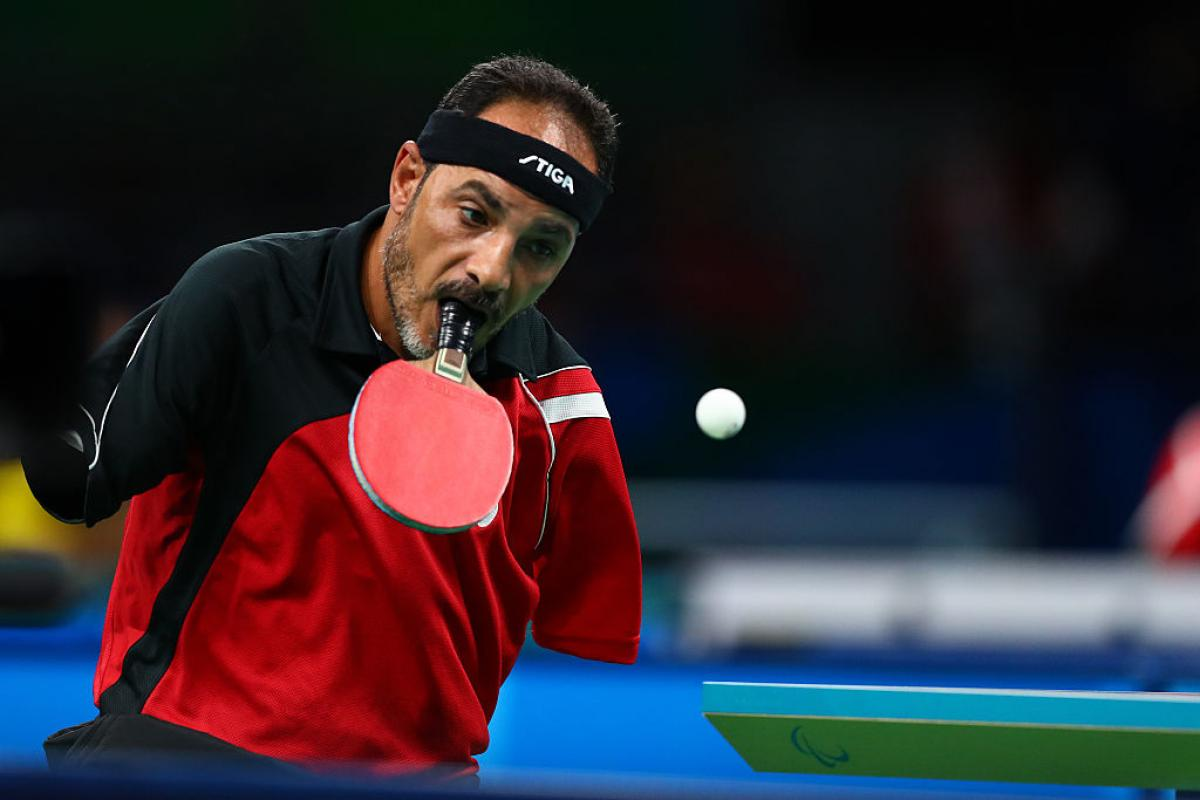
\includegraphics[width=0.8\textwidth]{Images/para_tabletennis.jpg}
\caption{Para Tabletennis}
\label{fig:my_image}
\end{figure}

\item Essence of Table Tennis
    \begin{itemize}
    \item Paralympic table tennis is a fast-paced and exhilarating sport that showcases the agility, reflexes, and tactical brilliance of athletes with various impairments. 
    \item Players compete in standing or wheelchair categories, battling each other across a table with small rackets and a lightweight ball. 
    \item The sport demands lightning-fast reactions, precise hand-eye coordination, and strategic shot placement, captivating spectators with its intensity and skill.
    \end{itemize}

\item Rules, Equipment, and Competition
    \begin{itemize}
    \item Paralympic table tennis adheres to the fundamental rules of table tennis, with adaptations made to accommodate different impairments. 
    \item The game is played in singles and doubles formats, and points are scored by hitting the ball onto the opponent's side of the table so that they cannot return it legally. 
    \item The sport utilizes a standard table tennis table, net, and balls, and athletes can use adaptive equipment like wheelchairs or prosthetic limbs based on their classification.
    \end{itemize}

\item Categories and Classifications
    \begin{itemize}
    \item Paralympic table tennis employs a classification system that groups athletes based on the impact of their impairment on their playing ability. 
    \item Athletes are categorized into different classes, with classes 1-5 for wheelchair users and classes 6-10 for standing players. 
    \item The classifications consider factors such as muscle power, range of movement, and balance, ensuring fair competition among athletes with similar functional abilities.
    \end{itemize}

\end{enumerate}
\subsection{Taekwondo}

\begin{enumerate}
\item Essence of Taekwondo
    \begin{itemize}
    \item Paralympic taekwondo is a dynamic and exciting martial art that showcases the power, precision, and agility of athletes with physical impairments affecting their lower limbs. 
    \item Standing on one leg, athletes deliver powerful kicks and punches to score points against their opponents. 
    \item The sport demands exceptional balance, coordination, and tactical awareness, demonstrating the remarkable adaptability and fighting spirit of athletes with disabilities.
    \end{itemize}

\item Rules, Equipment, and Competition
    \begin{itemize}
    \item Paralympic taekwondo follows the basic rules of taekwondo, with modifications to accommodate athletes with impairments. 
    \item Matches are contested in a standing position, with athletes wearing protective gear and scoring points by landing kicks and punches on designated target areas. 
    \item The competition format involves different weight categories and knockout rounds, culminating in thrilling finals where athletes battle for gold.
    \end{itemize}

\item Categories and Classifications
    \begin{itemize}
    \item Paralympic taekwondo currently includes only one sport class, K44, for athletes with impairments in their upper limbs. 
    \item However, the sport is continuously evolving, and future editions of the Games may include additional classifications to accommodate athletes with other impairments. 
    \item The current classification system ensures fair competition among athletes with similar functional abilities and allows them to showcase their taekwondo skills.
    \end{itemize}

\end{enumerate}
\subsection{Triathlon}

\begin{enumerate}

\item Essence of Triathlon
    \begin{itemize}
    \item Paralympic triathlon is the ultimate test of endurance and versatility, combining swimming, cycling, and running into a single, grueling event. 
    \item Athletes with various impairments showcase their strength, stamina, and determination as they navigate the challenging course, transitioning seamlessly between the three disciplines. 
    \item The sport celebrates the indomitable spirit of Paralympic athletes and their ability to push beyond limits.
    \end{itemize}

\item Rules, Equipment, and Competition
    \begin{itemize}
    \item Paralympic triathlon follows the core principles of triathlon, with adaptations for athletes with impairments. 
    \item The distances for each discipline vary depending on the classification, and athletes can use adaptive equipment such as handcycles, racing wheelchairs, or prosthetic limbs. 
    \item The competition format typically involves a continuous race, with athletes transitioning between the swim, bike, and run segments. 
    \end{itemize}

\item Categories and Classifications
    \begin{itemize}
    \item Paralympic triathlon features a classification system that groups athletes based on their impairment and functional abilities. 
    \item The system considers factors such as muscle power, range of movement, coordination, and balance. 
    \item Athletes are categorized into different classes, such as PTWC for wheelchair users, PTS for athletes with severe impairments who use prosthetics or assistive devices, and PTVI for visually impaired athletes who compete with a guide. 
    \item This classification ensures fair competition and allows athletes with diverse abilities to showcase their multi-sport skills.
    \end{itemize}

\end{enumerate}
\subsection{Wheelchair Basketball}

\begin{enumerate}

\item Essence of Wheelchair Basketball
    \begin{itemize}
    \item Wheelchair basketball is a fast-paced and exhilarating team sport that showcases the agility, skill, and teamwork of athletes with physical impairments affecting their lower limbs. 
    \item Players maneuver their wheelchairs with precision, dribbling, passing, and shooting the ball to score points against their opponents. 
    \item The sport is a dynamic blend of athleticism, strategy, and sheer determination, captivating audiences with its intensity and excitement.
    \end{itemize}

\item Rules, Equipment, and Competition
    \begin{itemize}
    \item Wheelchair basketball follows the core rules of basketball, with adaptations made for wheelchair users. 
    \item Players compete on a standard basketball court, using specially designed wheelchairs that allow for quick turns and maneuverability. 
    \item The game is played in four 10-minute quarters, and points are scored by shooting the ball through the hoop. 
    \item The sport demands exceptional ball-handling skills, teamwork, and strategic awareness, as players navigate the court and execute plays to outmaneuver their opponents.
    \end{itemize}

\item Categories and Classifications
    \begin{itemize}
    \item Wheelchair basketball utilizes a classification system that evaluates the athlete's functional abilities and assigns them a point value based on their trunk control, sitting balance, and ability to push and maneuver the wheelchair. 
    \item Players are grouped into teams with a maximum total point value, ensuring a balance of abilities on the court. 
    \item This system fosters fair competition and allows athletes with diverse impairments to participate and contribute to their team's success.
    \end{itemize}

\end{enumerate}
\subsection{Wheelchair Fencing}

\begin{enumerate}

\item Essence of Wheelchair Fencing
    \begin{itemize}
    \item Wheelchair fencing is a strategic and elegant combat sport that showcases the precision, agility, and tactical acumen of athletes with physical impairments. 
    \item Seated in wheelchairs that are securely fastened to the piste (fencing strip), athletes engage in duels using épée, foil, or sabre weapons, aiming to touch their opponents with the tip of their blade. 
    \item The sport demands lightning-fast reflexes, precise movements, and strategic thinking, creating a captivating display of skill and athleticism.
    \end{itemize}

\item Rules, Equipment, and Competition
    \begin{itemize}
    \item Wheelchair fencing adheres to the fundamental rules of fencing, with adaptations for athletes with impairments. 
    \item The wheelchairs are fixed to the piste, and athletes use modified grips and techniques to wield their weapons. 
    \item The competition format involves individual and team events, with fencers competing in different categories based on their weapon and classification. 
    \item Matches are won by scoring the most touches within a set time or reaching a certain number of points first.
    \end{itemize}

\item Categories and Classifications
    \begin{itemize}
    \item Wheelchair fencing utilizes a classification system based on the athlete's trunk control and fencing arm mobility. 
    \item There are two main categories: 
        \begin{itemize}
        \item Category A for athletes with good trunk control and fencing arm mobility
        \item Category B for those with limited trunk control or impaired fencing arm function
        \end{itemize} 
    \item This classification ensures fair competition and allows athletes with different levels of impairment to showcase their fencing skills and compete against others with comparable abilities.
    \end{itemize}

\begin{figure}[htbp] % htbp are float placement options
\centering
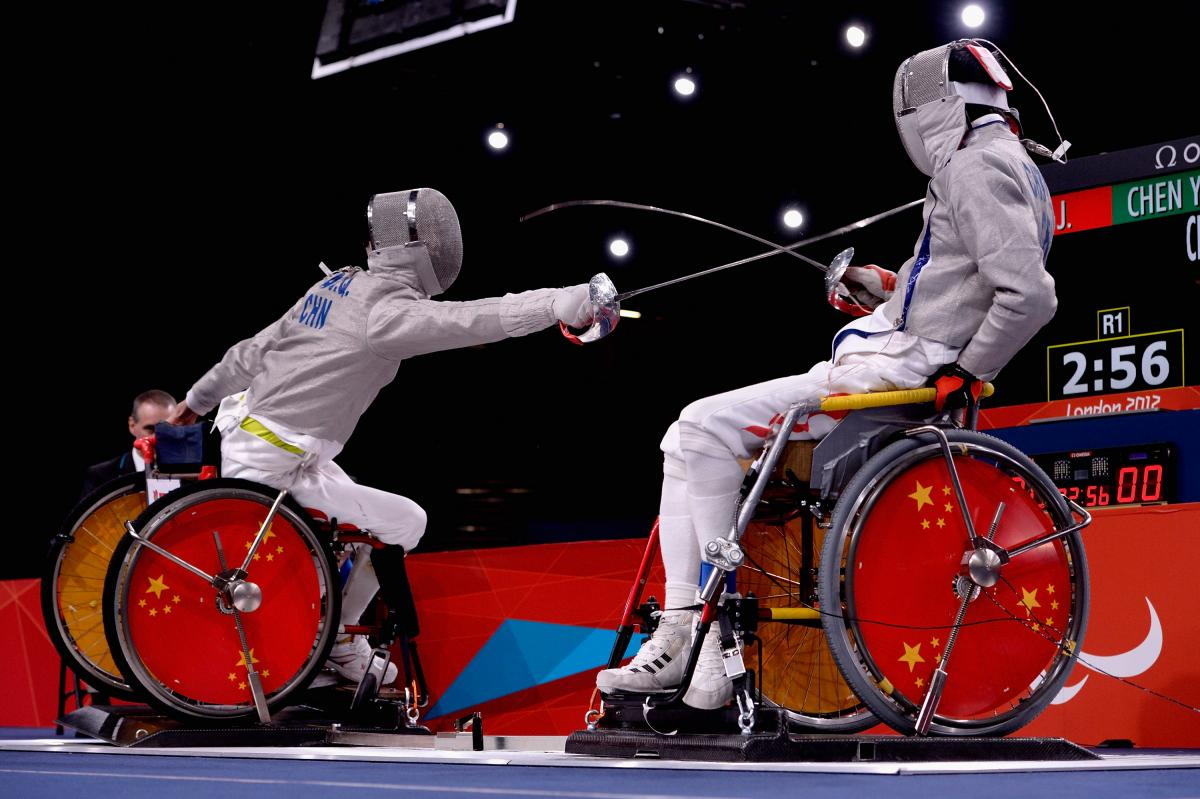
\includegraphics[width=0.8\textwidth]{Images/weelchair_fencing.jpg}
\caption{Weelchair fencing}
\label{fig:my_image}
\end{figure}

\end{enumerate}
\subsection{Wheelchair Rugby}

\begin{enumerate}

\item Essence of Wheelchair Rugby
    \begin{itemize}
    \item Wheelchair rugby, also known as "murderball," is a fast-paced and full-contact team sport that showcases the power, agility, and strategic brilliance of athletes with impairments affecting their limbs and trunk. 
    \item Played on a basketball court, athletes use specially designed wheelchairs to carry, pass, and dribble a volleyball across the opponent's goal line. 
    \item The sport is a thrilling spectacle of collisions, athleticism, and teamwork, demonstrating the resilience and competitive spirit of athletes with disabilities.
    \end{itemize}

\item Rules, Equipment, and Competition
    \begin{itemize}
    \item Wheelchair rugby combines elements of basketball, rugby, and handball, with modifications for wheelchair users. 
    \item Each team consists of four players, and the game is played in four 8-minute quarters. 
    \item Players use their wheelchairs to block and tackle opponents, creating a physically demanding and strategic game. 
    \item The sport utilizes specialized wheelchairs designed for durability and maneuverability, and athletes wear protective gear to minimize the risk of injury.
    \end{itemize}

\item Categories and Classifications
    \begin{itemize}
    \item Wheelchair rugby employs a unique classification system that assigns point values to athletes based on their functional abilities. 
    \item The system considers factors such as trunk control, arm and hand function, and overall mobility. 
    \item Each team is allowed a maximum number of points on the court at any given time, ensuring a balance of abilities and promoting fair competition among teams.
    \end{itemize}

\end{enumerate}
\subsection{Wheelchair Tennis}

\begin{enumerate}

\item Essence of Wheelchair Tennis
    \begin{itemize}
    \item Wheelchair tennis is a dynamic and exciting sport that showcases the agility, skill, and strategic prowess of athletes with physical impairments affecting their lower limbs. 
    \item Players compete in wheelchairs, using specially designed rackets to hit a tennis ball over a net. 
    \item The sport demands exceptional hand-eye coordination, quick reflexes, and tactical awareness, offering a thrilling spectacle of athleticism and competition.
    \end{itemize}

\item Rules, Equipment, and Competition
    \begin{itemize}
    \item Wheelchair tennis follows the same basic rules as able-bodied tennis, with the exception that the ball is allowed to bounce twice on the player's side of the court. 
    \item Players compete in singles and doubles formats, using standard tennis rackets and balls. 
    \item The competition format includes various tournaments and events, culminating in the prestigious Paralympic Wheelchair Tennis Championships. 
    \end{itemize}

\item Categories and Classifications
    \begin{itemize}
    \item Wheelchair tennis has two main categories: 
        \begin{itemize}
        \item Open division for athletes with impairments affecting their lower limbs
        \item Quad division for athletes with impairments affecting both their upper and lower limbs
        \end{itemize}
    \item This classification system ensures fair competition among athletes with similar functional abilities and allows them to showcase their tennis skills on a global stage
    \end{itemize}

\end{enumerate}